\section{系统边界与守恒条件}

把若干相互作用的物体作为一个系统，并不意味着这个系统的动量一定守恒。关键是系统边界外的物体在研究时间内提供了多少冲量。对各质点的动量定理相加，内部相互作用力成对抵消，得到$\bm P_2-\bm P_1=\int\bm F_{\text{外}}\dd t$。因此“系统不受合外力”保证其总动量在任意时刻不变；若只知道某一段的合外冲量为零，则只能保证该段始末动量相等。

分量守恒在竞赛中比完整的矢量守恒更常见。光滑水平面上物体的重力和支持力通常互相平衡，而墙、固定轴或绳的支点可能传递某个方向的外冲量。比如竖直摆绳处于最低点时，碰撞瞬间的绳冲量沿竖直方向，故球与入射物组成的系统可以沿水平守恒，却不能沿竖直守恒。画出外冲量的方向，才能决定保留哪一条分量方程。

\fig{fig:em2:pendulum-boundary}{固定支点能传外冲量：竖直绳在最低点约束竖直运动，水平分量仍可守恒}{\begin{tikzpicture}

\draw[world](-1,3)--(1,3);\draw[world](0,3)--(0,.3);\draw[world](0,0)circle(.3);
\draw[flow,blue](-2.7,0)--(-.6,0)node[midway,above]{$m\bm u$};\draw[world](-2.9,0)circle(.12);
\draw[guide](-3.3,-.6)rectangle(1.8,.7);\draw[force,red](0,.3)--(0,1.8)node[right]{$\bm J_{\text{支点}}$};
\draw[axis](.8,-.4)--(2,-.4)node[right]{$+x$};\node[right]at(.35,0){$M$};
\node at(-.4,-1.2){碰撞系统包括入射物和摆球，不包括固定支点};

\end{tikzpicture}}
图\ref{fig:em2:pendulum-boundary}的红色冲量穿过所选系统边界，它不能与球间内冲量一起消去。但它沿竖直绳方向，对$x$没有分量，所以可以单独使用$P_x$守恒。只有碰撞时绳竖直，这一“水平无约束冲量”的判断才直接成立；若在斜绳位置碰撞，应重新确定可守恒方向。


碰撞中的近似守恒还需要数量级条件。若碰撞时间为$\tau$，外部普通摩擦力为$f$，应检查$f\tau$远小于碰撞交换的典型动量。不能用“内力大”代替这个比较：若所求的动量变化本身很小，有限的外冲量仍可能重要。每次改变系统或改变时间区间，都要重新检查守恒条件。

\fig{fig:em2:boundary}{整体、子系统与可守恒分量}{\begin{tikzpicture}[scale=.9]\draw[guide](-.2,-.2)rectangle(5.6,2.2);\draw[world](.3,.4)rectangle(2,1.3);\node at(1.15,.85){$M$};\draw[world](3.5,.4)rectangle(5.2,1.3);\node at(4.35,.85){$m$};\draw[spring](2,.85)--(3.5,.85);\draw[force](1.1,.2)--(1.1,-.8)node[below]{$Mg$};\draw[force](1.1,1.5)--(1.1,2.5)node[above]{$N_M$};\draw[force](4.4,.2)--(4.4,-.8)node[below]{$mg$};\draw[force](4.4,1.5)--(4.4,2.5)node[above]{$N_m$};\node at(2.7,3.6){$F_{\text{外},x}=0\quad\Rightarrow\quad P_x=\text{常量}$};\end{tikzpicture}}

图\ref{fig:em2:boundary}虚线内两物体之间的弹力成对抵消，重力与支持力仍属于外力。图示条件只保证水平方向无外力，因而可令 $P_x$不变；改变系统边界或增加墙的水平冲量后，须重新审查该分量是否仍守恒。

\section{相对速度与质量加权平均}

所有动量相加以前，速度必须属于同一参考系。人从车上跳下时，“相对车的速度”为$u$，设车对地末速度为$V$，则人的对地末速度为$V+u$；不能把$u$直接放入地面系的动量式。若人、车初始共同以$v$运动，便有$(M+m)v=MV+m(V+u)$，由此$V=v-mu/(M+m)$。推导中质量较大的物体速度变化较小，正体现了相同反向冲量对不同质量的作用。

\fig{fig:em2:jump-relative}{初始静止的车与人反冲，人的对地速度与相对车速度不同}{\begin{tikzpicture}

\draw[world](0,0)rectangle(4,.4);\node at(2,.2){$M$};\draw[world](1.2,.4)--(1.2,1.5);\draw[world](1.2,1.75)circle(.25);\node[left]at(.8,1.1){$m$};
\draw[flow,blue](0,-.6)--(-1.3,-.6)node[midway,below]{$V<0$};
\draw[flow,blue](1.2,2.4)--(3,2.4)node[midway,above]{$v_p=V+u>0$};
\draw[axis](5,-.1)--(6.4,-.1)node[right]{$+x$};
\draw[dim](-1.3,3.5)--(1.8,3.5)node[midway,above]{$u=v_p-V$};\node at(2,-1.5){初始静止时：$MV+m(V+u)=0$};

\end{tikzpicture}}
图\ref{fig:em2:jump-relative}选取初始静止的情形，车向后、人与车的相对运动向前。两者对地速度代入动量式；给定的$u$则用来联系两个末速度。若把$u$直接作为人的对地速度，就会把车的反冲速度漏算一次。


两物体最终相对静止时，共同速度由$V=(m_1v_1+m_2v_2)/(m_1+m_2)$决定。它是有符号速度的质量加权平均，不是速率的平均。这个结果与内部经历几次碰撞、摩擦多久无关，只要求相应方向的外冲量可忽略。若从相向运动开始，先规定正方向，再把反向初速度写成负值，便可直接判定共同运动方向。

共同速度只说明相对速度为零。它可能发生在永久粘合之后，也可能仅发生在弹簧压缩至最短的一瞬间；应继续检查能量存储与耗散的机制。

两物体的速度可统一分成“质心运动”和“相对运动”。设$M_\Sigma=m_1+m_2$、$u=v_1-v_2$，由$m_1v_1+m_2v_2=M_\Sigma V_C$及$v_1-v_2=u$联立，先将$v_1=v_2+u$代入第一式，得$v_2=V_C-m_1u/M_\Sigma$，再得
\[v_1=V_C+\frac{m_2}{M_\Sigma}u,\qquad v_2=V_C-\frac{m_1}{M_\Sigma}u.\]
它们不是额外的守恒定律，而是动量定义与相对速度定义的联立结果；内部作用改变$u$，外部合冲量决定$V_C$怎样变化。两者在解题中的作用因而可以分开。

\fig{fig:em2:same-speed}{同速条件相同，弹簧储能与非弹性粘合的能量去向不同}{\begin{tikzpicture}

\begin{scope}
\draw[world](0,0)rectangle(1,.7);\draw[world](2,0)rectangle(3,.7);\draw[spring](1,.35)--(2,.35);
\draw[flow,blue](.2,1.2)--(1.2,1.2)node[above]{$V_C$};\draw[flow,blue](2.2,1.2)--(3.2,1.2)node[above]{$V_C$};
\node at(1.5,-.7){弹簧最压缩，$u=0$};\node at(1.5,-1.4){相对运动能量暂存为弹性势能};
\end{scope}
\begin{scope}[xshift=6.4cm]
\draw[world](0,0)rectangle(2,.7);\draw[guide](1,0)--(1,.7);\node at(1,.35){粘合体};
\draw[flow,blue](.5,1.2)--(1.5,1.2)node[above]{$V_C$};
\node at(1,-.7){永久粘合，$u=0$};\node at(1,-1.4){相对运动能量转为内能等};
\end{scope}
\end{tikzpicture}}
图\ref{fig:em2:same-speed}中若合外冲量为零，$V_C$始终固定。把前面的两个速度表达代入$K=m_1v_1^2/2+m_2v_2^2/2$，逐项展开：
\begin{align*}
K={}&\frac12(m_1+m_2)V_C^2
+\left(\frac{m_1m_2}{M_\Sigma}-\frac{m_2m_1}{M_\Sigma}\right)V_Cu\\
&+\frac12\frac{m_1m_2^2+m_2m_1^2}{M_\Sigma^2}u^2.
\end{align*}
交叉项为零，最后一项的系数中$m_1m_2^2+m_2m_1^2=m_1m_2M_\Sigma$，约去一个$M_\Sigma$，得到
\[
K=\frac12M_\Sigma V_C^2+\frac12\mu_r u^2,
\qquad \mu_r=\frac{m_1m_2}{m_1+m_2}.
\]
第一项是质心运动的动能，第二项随相对速度改变。弹簧压缩时第二项可变成弹性势能，粘合时它可转为内能；这一分解本身不附加任何能量守恒假设。


\section{选择参考系时守恒式怎样变化}

两个惯性系以恒定速度$U$相对平动时，各物速度都减去$U$，系统总动量变为$P'=P-M_{\Sigma}U$。质量固定且外冲量为零时，两个系都能写动量守恒，因为减去的是同一个常量。相对速度不变，也使恢复系数在伽利略变换下保持不变。动能则须把每个速度的平方完整展开：
\[
K'=\frac12\sum_i m_i(v_i-U)^2
=\frac12\sum_i m_iv_i^2-U\sum_i m_iv_i+\frac{U^2}{2}\sum_i m_i
=K-UP+\frac12M_\Sigma U^2.
\]
所以动能数值本身随参考系变化。

\fig{fig:em2:galilean}{更换惯性系使两速度同时减去$U$，速度差保持不变}{\begin{tikzpicture}

\begin{scope}
\draw[axis](-1.7,0)--(4.4,0)node[right]{$v$};\fill(1,0)circle(2pt)node[above]{$v_2$};\fill(3,0)circle(2pt)node[above]{$v_1$};
\draw[dim](1,-.6)--(3,-.6)node[midway,below]{$u=v_1-v_2$};\node[left]at(-1.7,0){$S$系};
\end{scope}
\node at(1.2,-1.4){所有速度统一减去$U$};
\begin{scope}[yshift=-2.5cm]
\draw[axis](-1.7,0)--(4.4,0)node[right]{$v'$};\fill(-1,0)circle(2pt)node[above]{$v'_2$};\fill(1,0)circle(2pt)node[above]{$v'_1$};
\draw[dim](-1,-.6)--(1,-.6)node[midway,below]{$u'=u$};\node[left]at(-1.7,0){$S'$系};
\end{scope}
\end{tikzpicture}}
图\ref{fig:em2:galilean}在速度数轴上表示同一变换，正负号都随统一平移改变，但两速度间距不变。动量的变换也应对所有物质采用同一个$U$：$P'=\sum_i m_i(v_i-U)=P-M_\Sigma U$，不能只转换其中一个物体。


对于孤立碰撞，初、末总动量相同，故动能损失$K_i-K_f$在这些惯性系中相同。这说明“某物动能增加多少”会随参考系改变，而整个孤立碰撞的机械能损失不会因此改变。涉及运动船上抛球和自由发射器的题中，先选地面惯性系写守恒，再用相对速度表示末态，通常比在正在反冲的车系直接套用守恒更清楚。

并非所有方便的坐标系都是惯性系。小车在发射期间加速，其瞬时车系不能直接当成全程惯性系；若确需在车系列动力学，必须加入惯性力及其功。这里用速度变换只是把同一瞬间的相对速度换算为地面速度，并未把车系作为全程列守恒的参考系。

\section{质心定理与位移关系}

系统的质心位置定义为$\bm R_C=\sum m_i\bm r_i/M_{\Sigma}$。在质量不变时对时间求导，得到$M_{\Sigma}\bm V_C=\sum m_i\bm v_i=\bm P$；再求导，得到$M_{\Sigma}\bm A_C=\bm F_{\text{外}}$。因此总动量守恒时，质心保持匀速直线运动。初始总动量为零，质心位置才不变，不能把“动量守恒”直接说成“质心静止”。

对两物体沿水平方向，若质心速度为$V_C$，在时间$T$内有$m\Delta x+M\Delta X=(m+M)V_CT$。如果另已知两物体的相对位移$\Delta x-\Delta X=\ell$，先将$\Delta x=\Delta X+\ell$代入第一式，得$(M+m)\Delta X+m\ell=(M+m)V_CT$；移项、除以总质量，再代回相对位移式，得到
\[\Delta X=V_CT-\frac{m}{M+m}\ell,\qquad \Delta x=V_CT+\frac{M}{M+m}\ell.\]
人船、球与活动槽、板上滑动物体的问题，往往只需这一位移关系，不必求整个加速过程。图中必须区分对地位移与相对位移：相对船走了一个船长，并不表示人在地面系也走了一个船长。

\fig{fig:em2:cm}{质心匀速运动与相对位移}{\begin{tikzpicture}[scale=.9]\draw[world](0,1)--(4,1);\fill(0,1.15)circle(.06)node[above]{$m$};\node at(2,1.35){$M$};\draw[world](-1,-.5)--(3,-.5);\fill(3,-.35)circle(.06)node[above]{$m$};\node at(1,-.15){$M$};\draw[flow](0,.55)--(3,.55)node[midway,above]{$\Delta x$};\draw[flow](0,-1)--(-1,-1)node[midway,below]{$\Delta X$};\draw[guide](1.5,1.8)--(1.5,-1.25);\node at(1.5,2.2){示意取$M=3m$，$X_C$固定};\end{tikzpicture}}

图\ref{fig:em2:cm}中的质心位置由质量加权确定。内部移动时，用同一地面系量出各物体位移，再令其质量加权和等于总质量乘质心位移。初始总动量为零时质心固定；初始总动量非零时，应保留质心的匀速位移。


这一表达对中间是否停顿、是否先向反方向走均不敏感，但它不能替代所需时间或最大速度的动力学计算。若人走到船头再回船尾，最终$\ell=0$，船只保留原有的匀速平移；若人在船头停下，船则留下一个与$m\ell$成比例的相对位移。这样可以把“速度回到原值”和“位置回到原处”区分开。

\section{连续体质心的积分计算}

质心定义中的质量加权和，对连续分布应写成$\bm R_C=M^{-1}\int\bm r\dd m$。积分前先确定质量微元：细杆用$\dd m=\lambda(x)\dd x$，薄片用$\dd m=\sigma(x,y)\dd A$，立体用$\dd m=\rho(x,y,z)\dd V$。若密度不均匀，不能把几何中心直接当成质心；如果有对称面，质心必在该面上，这通常能先消去一个或两个未知坐标。

例如长$\ell$的细杆沿$x\in[0,\ell]$放置，线密度$\lambda(x)=\lambda_0(1+x/\ell)$。右端更重，质心应在中点右侧。总质量和关于左端的一阶矩分别为
\[
M=\lambda_0\int_0^\ell(1+x/\ell)\dd x
=\lambda_0\left[x+\frac{x^2}{2\ell}\right]_0^\ell
=\lambda_0(\ell+\ell/2)=\frac32\lambda_0\ell,
\]
\[
Mx_C=\lambda_0\int_0^\ell(x+x^2/\ell)\dd x
=\lambda_0\left[\frac{x^2}{2}+\frac{x^3}{3\ell}\right]_0^\ell
=\lambda_0\ell^2\left(\frac12+\frac13\right)=\frac56\lambda_0\ell^2.
\]
所以$x_C=5\ell/9$，满足先前的方向判断。积分中分母的$M$也应由同一密度函数算出，不能一面使用非均匀密度求矩，一面仍写$M=\lambda_0\ell$。

\fig{fig:em2:density}{非均匀杆按当地线密度取微元，三角薄片按随高度变化的条带取微元}{\begin{tikzpicture}

\begin{scope}
\shade[left color=blue!8,right color=blue!55](0,-.16)rectangle(4,.16);\draw[world](0,-.16)rectangle(4,.16);
\draw[fill=red!30](2.7,-.16)rectangle(2.9,.16);\node[above]at(2.8,.4){$\lambda(x)\dd x$};
\fill(2.222,0)circle(2pt)node[below]{$C$};\node[below]at(0,0){$0$};\node[below]at(4,0){$\ell$};
\node at(2,1.4){$\lambda=\lambda_0(1+x/\ell)$};\draw[dim](0,-.8)--(2.8,-.8)node[midway,below]{$x$};
\end{scope}
\begin{scope}[xshift=6.2cm]
\draw[world](0,0)--(3,0)--(1.5,3)--cycle;
\draw[fill=blue!20](.6,1.2)--(2.4,1.2)--(2.3,1.4)--(.7,1.4)--cycle;
\node[right]at(2.4,1.3){$b(1-y/H)$};\node[left]at(.6,1.3){$\dd y$};
\draw[dim](-.7,0)--(-.7,3)node[midway,left]{$H$};\draw[dim](0,-.6)--(3,-.6)node[midway,below]{$b$};
\fill(1.5,1)circle(2pt)node[below]{$C$};
\end{scope}
\end{tikzpicture}}

图\ref{fig:em2:density}右侧的均匀三角薄片，底边位于$y=0$、顶点位于$y=H$。高度$y$处条带宽度为$b(1-y/H)$，质量微元$\dd m=\sigma b(1-y/H)\dd y$。从底边积到顶点，
\begin{align*}
M&=\sigma b\int_0^H(1-y/H)\dd y
=\sigma b[y-y^2/(2H)]_0^H=\frac{\sigma bH}{2},\\
My_C&=\sigma b\int_0^H(y-y^2/H)\dd y
=\sigma b[y^2/2-y^3/(3H)]_0^H\\
&=\sigma bH^2(1/2-1/3)=\frac{\sigma bH^2}{6}.
\end{align*}
两式相除，$y_C=(H^2/6)/(H/2)=H/3$。条带的宽度进入质量微元，这一方法也适用于密度随高度改变的薄片。

组合物体也可把各部分当成位于自身质心的质量来计算总质心。对挖孔薄片，数学上可以用完整薄片减去被挖去部分的一阶矩，但分母必须是剩余总质量。负号表示扣除质量，并非存在负质量物体。求出后应检查结果是否向缺孔相反方向偏移；形状图提供的是有意义的物理检验。
\fig{fig:em2:hole-moment}{挖去右侧质量后，剩余质心向左偏移；负号表示扣除一阶矩}{\begin{tikzpicture}

\fill[blue!10](0,0)circle(2);\fill[white](1,0)circle(.85);\draw[world](0,0)circle(2);\draw[world](1,0)circle(.85);
\draw[guide](-2.4,0)--(2.4,0);\fill(0,0)circle(2pt);\draw[guide](0,0)--(-.1,-.9)node[below]{$O$};
\fill(1,0)circle(2pt)node[right]{$C_h$};\fill(-.2204,0)circle(2pt);\draw[guide,red](-.2204,0)--(-1.1,.8)node[left]{$C$};
\node[align=left]at(5,1){完整质量$M_0$，孔内质量$m_h$\\$(M_0-m_h)\bm r_C=M_0\bm r_O-m_h\bm r_h$};
\node[align=left]at(5,-.6){图中$\bm r_O=0$、$x_h>0$\\所以$x_C=-m_hx_h/(M_0-m_h)<0$};

\end{tikzpicture}}
图\ref{fig:em2:hole-moment}先把完整圆片和孔内圆片分别归结到各自质心，分母则使用剩余质量$M_0-m_h$。质心向孔的反侧移动，给计算提供一个无需积分的方向检查；对不规则孔，须先求孔内部分本身的质心。


\section{质心高度与均匀重力场}

在均匀重力场中，各质元重力相同方向，重力势能总和为$U_g=\int gy\dd m=MgY_C$。因此整体变形或内部移动的重力功，可以只由质心高度变化计算：$W_g=-Mg\Delta Y_C$。这并不是把刚体各点的真实运动都替换成质心运动，而只是利用均匀重力场使势能对高度呈线性。

\fig{fig:em2:gravity-center}{均匀杆放倒时端点降低$L$，全杆质心只降低$L/2$}{\begin{tikzpicture}

\draw[world](-.5,0)--(4,0);\draw[world,line width=1.5pt](0,0)--(0,3);
\draw[world,line width=1.5pt,dashed](0,0)--(3,0);
\fill(0,1.5)circle(2pt)node[left]{$C_i$};\fill(1.5,0)circle(2pt)node[below]{$C_f$};
\draw[dim](-.8,0)--(-.8,3)node[midway,left]{$L$};\draw[dim](.6,0)--(.6,1.5)node[midway,right]{$L/2$};
\draw[axis,blue](0,2.3)arc(90:5:2.3);\node[right]at(3,1.3){$W_g=MgL/2$};

\end{tikzpicture}}
图\ref{fig:em2:gravity-center}中每个质元的下降高度不同。以杆下端为原点，初态$Y_C=L/2$，末态$Y_C=0$，故重力作功$MgL/2$。只取上端下降高度$L$写成$MgL$，等于误把全杆质量集中在上端。


链条被提起、液体被排出、杆由竖直到水平，均可用这一关系检查逐微元积分。若只给末端上升的高度，尚不足以直接写$Mgh$，因为并非每个质元都上升同样高度；应先求整个物体质心变化。另一方面，在非均匀引力场中，重力不再对所有质元同样，通常不能把相互作用能严格写成一个集中质量的近地表达式，需回到适当的势能积分。

\section{质心坐标与事件的独立性}

质心法消去内部运动细节，并不意味着内部细节对所有问题都无关。人船题中，只要初、末相对位置已知，就可直接求船位移；若改求最大速度、行走所需功或船受到的瞬时作用力，还必须知道行走方式。计算时应先辨认问题只依赖状态，还是还依赖过程，避免把质心法能处理的范围过度扩大。

若系统由多个活动部分组成，可选一个公共基体位移$X$，每个物体的对地位移表示为$X+\ell_i$。质心关系变成$M_{\Sigma}X+\sum m_i\ell_i=M_{\Sigma}V_CT$。这个表达不需要知道实际质心在哪里，因而在人互换位置、两船交换载荷和连续接收物体时尤其方便。若物质最终离开系统，就要把离开物也保留在最初所选的物质系统内，或者明确加入其带走的动量流。

\fig{fig:em2:explosion-center}{爆炸只改变内部相对运动，触地前两碎片的质心仍沿原抛物线运动}{\begin{tikzpicture}

\draw[world](-1,0)--(4.3,0);\draw[world,blue,domain=-.8:1.777,samples=70]plot(\x,{3-.5*(\x)^2});
\fill(0,3)circle(2pt)node[below left]{$E$};\draw[flow](0,3)--(1,3)node[above]{$v_x$};
\draw[world,red,domain=0:1.777,samples=60]plot({2*\x},{3-.8*\x-.5*(\x)^2});
\draw[guide](0,3)--(0,3.32);\fill(0,3.3)circle(2pt)node[above left]{$m_1$};
\fill(2,1.7)circle(2pt)node[right]{$m_2$};\draw[guide](0,3.3)--(2,1.7);
\fill(1,2.5)circle(2pt)node[above right]{$C$};\fill(3.554,0)circle(2pt)node[above right]{首次触地};
\node[align=left]at(6.6,2.6){图示两片质量相等\\同一时刻$C$为两片中点\\蓝线为未爆炸的轨迹};
\node at(1.2,-.9){首次触地后，地面冲量必须计入};

\end{tikzpicture}}
图\ref{fig:em2:explosion-center}用等质量两碎片示意质心位置：连接同一时刻的两碎片，中点$C$仍在蓝线上。它约束的是全部碎片的加权位置，并未要求每片各自沿原轨迹运动。这个结论也有明确的终止事件。


用质心追踪爆炸后的物体时，只有全部碎片都仍受相同重力场且可忽略空气阻力，系统质心才沿未爆炸物体的轨迹继续运动。某个碎片撞地后，地面提供额外外冲量，质心轨迹立即改变。因此应先找到第一片触地的时刻，再判断能否把质心抛体结论继续用于后面的阶段。

\section{内部摩擦与动量交换}
物块滑上自由木板时，摩擦对物块向后、对木板向前。两摩擦冲量在整体动量式中抵消，却分别改变两个速度。设物块质量$m$、初速度$v_0$，木板质量$M$、初始静止，滑动摩擦力大小$f=\mu mg$。在物块仍相对木板向前滑动的阶段，
\[
v_m=v_0-\frac fm t,\qquad v_M=\frac fM t,
\qquad u(t)=v_m-v_M=v_0-f\left(\frac1m+\frac1M\right)t.
\]
令$u(t_*)=0$，得共速时间$t_*=mMv_0/[f(M+m)]$。在此之前$u>0$，验证了所用摩擦方向；共速并不等于物块对地静止，它们的共同速度为$mv_0/(M+m)$。

判断物块是否滑出，应积分相对速度，不能只算物块对地位移：
\[
\ell_{\text{相}}=\int_0^{t_*}\left(v_0-\frac{v_0}{t_*}t\right)\dd t
=\left[v_0t-\frac{v_0t^2}{2t_*}\right]_0^{t_*}
=v_0t_*-\frac12v_0t_*=\frac12v_0t_*.
\]
若板上可用长度小于$\ell_{\text{相}}$，物块先到达板端，摩擦模型须在离板时截断，预设的共速状态并未实现。图\ref{fv:e2:slip}将摩擦方向与这一面积判据放在同一组图中。

\fig{fv:e2:slip}{摩擦反向交换动量，相对速度图的面积决定是否滑出木板}{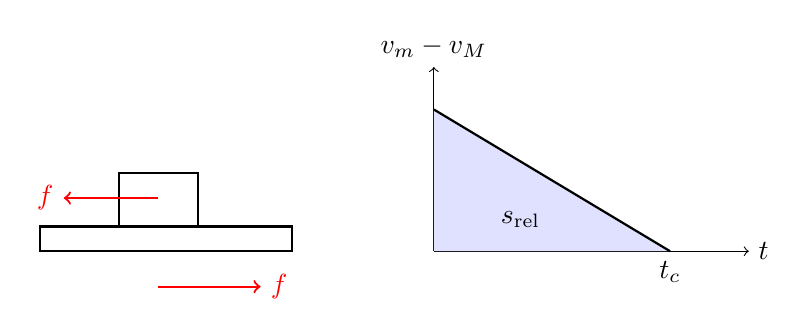
\begin{tikzpicture}[x=1cm,y=.9cm]
\draw[thick](0,0)rectangle(3.2,.35);\draw[thick](1,.35)rectangle(2,1.1);
\draw[->,red,thick](1.5,.75)--(.3,.75)node[left]{$f$};\draw[->,red,thick](1.5,-.5)--(2.8,-.5)node[right]{$f$};
\begin{scope}[xshift=5cm]\draw[->](0,0)--(4,0)node[right]{$t$};\draw[->](0,0)--(0,2.6)node[above]{$v_m-v_M$};
\fill[blue!12](0,0)--(0,2)--(3,0)--cycle;\draw[thick](0,2)--(3,0);\node[below]at(3,0){$t_c$};\node at(1.1,.45){$s_{\rm rel}$};\end{scope}
\end{tikzpicture}}
图\ref{fv:e2:slip}左侧两摩擦力属于不同物体，所以在整体动量式中相消，在各自方程中却都要保留。右侧画的是相对速度，蓝色面积 $s_{\rm rel}=\int_0^{t_c}(v_m-v_M)\dd t$才是物块在板上走过的长度。对地位移中还包含板的运动，不能直接拿它与板长比较。若板端先被到达，共速条件尚未实现，便须提前结束这段摩擦模型。


\section{变质量喷射与封闭系统}

火箭的推力来自喷出物的动量变化。设火箭质量为$M$、速度为$V$，短时间内喷出正质量$\delta m$，喷气相对火箭向后速度为$u$。忽略二阶量，在地面系中，喷气的速度应写成$V-u$，而不是$-u$。选“喷气前的整个火箭”为封闭系统，有
\[MV=(M-\delta m)(V+\dd V)+\delta m(V-u).\]
把右边的两个乘积展开，$MV+M\dd V-V\delta m-\delta m\dd V+V\delta m-u\delta m$中，两项$V\delta m$相消；再约去$MV$，得
\[
M\dd V-u\delta m-\delta m\dd V=0.
\]
舍去二阶乘积$\delta m\dd V$，所以$M\dd V=u\delta m$。
因$\dd M=-\delta m$，故$\dd V=-u\dd M/M$。若无外力、$u$为常量，质量从 $M_0$ 降到 $M$，速度从 $V_0$ 升到 $V$，有
\[
\int_{V_0}^{V}\dd W=-u\int_{M_0}^{M}\frac{\dd\mu}{\mu}.
\]
换元 $q=\mu/M_0$，则 $\dd\mu/\mu=\dd q/q$，上下限变为 $1,M/M_0$，所以
\[
V-V_0=-u[\ln q]_1^{M/M_0}
=-u\ln(M/M_0)=u\ln(M_0/M).
\]
初始条件与积分端点已确定常数。有外力时应在短时动量式中加入外冲量，不能先宣布火箭自身动量守恒。

\fig{fig:em2:rocket-element}{在短时间内把喷出燃料也保留在封闭系统中，统一使用地面速度}{\begin{tikzpicture}

\begin{scope}
\draw[guide](-.4,-.5)rectangle(3.5,1.8);\draw[world](.4,0)rectangle(2.4,.8);\node at(1.4,.4){$M$};
\draw[flow](2.5,.4)--(3.6,.4)node[right]{$V$};\node at(1.5,-1){喷气前};
\end{scope}
\begin{scope}[xshift=6cm]
\draw[guide](-1.4,-.5)rectangle(3.5,1.8);\draw[world](.4,0)rectangle(2.4,.8);\node at(1.4,.4){$M-\delta m$};
\fill(-.7,.4)circle(.08)node[below]{$\delta m$};\draw[flow,red](-.7,.9)--(-1.8,.9)node[left]{$u$，相对火箭};
\draw[flow](2.5,.4)--(3.7,.4)node[right]{$V+\dd V$};\node at(.7,-1){燃料对地速度$V-u$};
\end{scope}
\end{tikzpicture}}
图\ref{fig:em2:rocket-element}中的虚线前后圈住同一批物质。喷气后的火箭质量减少，而燃料仍有对地动量$\delta m(V-u)$；只保留火箭本身就会漏掉这部分。相对喷速$u$用于速度换算，不能直接把燃料对地速度写成$-u$。


“系统”也可以包含外部装置。风扇向船帆吹风时，只算帆受到的推力会漏掉风扇的反作用。若气流最终仍留在船上，内部冲量可能完全抵消；若气流离船时仍带走定向动量，船才得到相反的总动量。决定装置推进效果的是边界上的最终动量流，而不是某一局部的压力大小。

若要与一次抛出比较，必须说明“相对喷出速率”相对哪一个末态。假设初始质量$M_0$，一次抛出燃料$M_0-M$，燃料相对最终火箭向后速率仍为$u$，则燃料对地速度为$V-u$。动量式$M_0V_0=MV+(M_0-M)(V-u)$给
\[V-V_0=u\left(1-\frac{M}{M_0}\right).\]
连续喷射则给$u\ln(M_0/M)$。令质量比$r=M_0/M>1$，比较函数$D(r)=\ln r-1+1/r$。有
\[
D(1)=0,\qquad D'(r)=\frac1r-\frac1{r^2}=\frac{r-1}{r^2}>0.
\]
所以$D(r)>0$，即$\ln r>1-1/r$。在这项相同相对喷速的约定下，连续喷射的速度增量较大。比较并不代表二者所耗能量相同；只给相对喷速，不能同时擅自要求输入能量也相等。

